
\documentclass[10pt, a4paper, twoside]{article}
\usepackage[utf8]{inputenc}
\usepackage{newtxtext,newtxmath} % Times New Roman font
\usepackage[left=2.54cm, right=2.54cm, top=2.54cm, bottom=2.54cm, headheight=15pt]{geometry}
\usepackage{titlesec} % For customizing section titles
\usepackage{enumitem} % Enables bullet points
\usepackage{lipsum} % Add dummy text
\usepackage{hyperref} % Links for references
\usepackage{parskip} % Set spacing between paragraphs
\usepackage{fancyhdr} % Format headers
\usepackage{etoolbox} % Format bibliography header
\usepackage{siunitx} % Used to write SI base units
\usepackage{physics} % Used to write differential equations more easily
\usepackage{graphicx} % Used for figures
\usepackage{caption} % Used to edit the figure captions
\usepackage{ulem} % Enables strikethrough text with \sout command.

% This code is used to supress \qty warning conflict between siunitx and physics packages
% \ExplSyntaxOn
% \msg_redirect_name:nnn { siunitx } { physics-pkg } { none }
% \ExplSyntaxOff

\setlength{\parskip}{10pt}

\titleformat{\section}{\normalfont\fontsize{10}{13}\uppercase}{\thesection.}{1em}{}
\titleformat{\subsection}{\normalfont\fontsize{10}{13}\bfseries}{\thesubsection.}{1em}{}
\titleformat{\subsubsection}{\normalfont\fontsize{10}{13}\itshape}{\thesubsubsection.}{1em}{}

% Redefining \section* command for centered section title
\titleformat{name=\section,numberless}{\normalfont\fontsize{10}{13}\bfseries\centering\uppercase}{}{0pt}{}

% Ensure references title has the same format as \section*
\patchcmd{\thebibliography}{\section*{\refname}}{\section*{REFERENCES}}{}{}

%  Create headers and footers
\fancyhf{} % clear all header and footer fields
\renewcommand{\headrulewidth}{0pt}
% \fancyhead[CE]{\fontsize{8}{10}\selectfont \textbf{IAEA-CN-316/2143}}
\fancyhead[CE]{\fontsize{8}{10}\selectfont \textbf{CONFINEMENT OF ALPHAS IN STEP}}
\fancyhead[CO]{\fontsize{8}{10}\selectfont \textbf{PROKOPYSZYN et al.}}
\fancyfoot[RO]{\fontsize{10}{13}\selectfont \thepage}
\fancyfoot[RE]{\fontsize{10}{13}\selectfont \thepage}
\pagestyle{fancy}

% Set the caption font size to 9pt
\DeclareCaptionFont{ninept}{\fontsize{9pt}{12pt}\selectfont}
\renewcommand{\figurename}{\textit{FIG.}}
\captionsetup{
    justification=raggedright,
    singlelinecheck=true,
    font=ninept,
    textfont=it,
    labelfont=it,
    labelsep=period,
    labelformat=simple,
    format=hang
}

\begin{document}
\begin{flushleft}
\fontsize{12}{14}\selectfont \textbf{CONFINEMENT OF FUSION ALPHA-PARTICLES AND ALFV\'EN EIGENMODE STABILITY IN STEP}
% \fontsize{12}{14}\selectfont \textbf{\textit{Subtitle if needed in Times New Roman 12 point bold italic, sentence case}}

\fontsize{10}{13}\selectfont
A.P.K. PROKOPYSZYN, K.G. MCCLEMENTS, H.J.C. OLIVER, M. FITZGERALD, D.A. RYAN, G. XIA \\
United Kingdom Atomic Energy Authority \\
Culham Campus, Abingdon, Oxfordshire OX14 3DB, United Kingdom \\
Email: alex.prokopysyzn@ukaea.uk

\end{flushleft}

% Abstract section
\begin{flushleft}
\textbf{Abstract}
\end{flushleft}

\setlength{\parindent}{1cm}
\fontsize{9}{12pt}\selectfont

The Spherical Tokamak for Energy Production (STEP) programme is focused on designing and building a prototype fusion power plant that will generate approximately 1.5-1.8 GW of deuterium-tritium fusion power. To achieve this, the $\alpha$-particles generated through fusion must be adequately confined to maintain the necessary high temperature in the core of the plasma and to protect the wall from too much damage. Microwaves will be used for both external heating and current drive, making $\alpha$-particles the only significant fast-ion species. The purpose of this work is to model the confinement of $\alpha$-particles and the toroidal Alfvén eigenmodes (TAEs) driven by these particles in a variety of scenarios to help determine the best configuration. The scenarios examined here have been identified by the STEP team as potential flat-top operating configurations. We use LOCUST (Lorentz Orbit Code for Use in Stellerators and Tokamaks) to model the $\alpha$-particle confinement and heat-load distribution on the wall, and HALO (HAgis LOcust) to model the TAEs. The results indicate that acceptable confinement in terms of power loading can be achieved in candidate flat-top operating points, but the results are sensitive to some of the system parameters. For example, a change in the phase difference between the upper and lower edge localised mode (ELM) suppression coils can increase the maximum power load on the first wall due to $\alpha$ particle losses by a factor of 10.

% Abstract and title over, format text for the main body
\setlength{\parindent}{0pt}
\fontsize{10}{13}\selectfont

\section{Introduction}
\label{sec:introduction}

UKAEA is pioneering efforts to develop a compact prototype of a fusion energy power plant and establish a commercial pathway for fusion energy \cite{nuttall2020, meyer2023, mitchell2023}. A crucial factor in the viability of a deuterium-tritium (D-T) burning fusion reactor is the confinement of fusion-born $\alpha$-particles since, in addition to providing most of the plasma heating, these particles have the potential to damage the reactor walls when unconfined. Ideally, $\alpha$-particles should slow down through Coulomb collisions with thermal electrons and ions while undergoing a modest level of (purely collisional) transport. However, they can drive high-frequency instabilities that, in turn, can transport them at rates well above collisional levels \cite{garcia-munoz2011}. Toroidal Alfv\'en eigenmodes (TAEs) exemplify the type of fast particle-driven instability that can significantly disrupt plasma confinement. In the present work we model $\alpha$-particle losses in the presence of static magnetic fields and determine the stability of TAEs in candidate STEP plasmas with the objective of informing the design process for this device.

External heating and current drive for the plasma in STEP during the flat-top configuration will be provided entirely by microwaves. This heating strategy will utilise a combination of electron cyclotron current drive and electron Bernstein waves. Detailed information on the proposed heating and current drive systems for STEP is provided in \cite{Henderson2024}.
This approach has significant implications, as it means that the only substantial population of fast ions will be composed of $\alpha$-particles, which are a product of the fusion reaction itself. Unlike other tokamak devices such as JET and ITER, STEP will not generate fast ions via neutral beam injectors or ion cyclotron resonance heating systems.
In this context, `fast ions' are defined as ions with speeds that are significantly greater than those of the background plasma, making them suprathermal. For example, in the STEP design, the plasma at the core is expected to reach a temperature of approximately 20 keV (see, e.g. \cite{meyer2023,mitchell2023}), whereas the fusion-born $\alpha$-particles will be born with energies of around 3.5 MeV, much higher than the background plasma.

The commercial viability of STEP will rely on the longevity of the plasma-facing components. During operation, the PFCs will be exposed to heat from various sources, even if disruptions are successfully avoided. The wall will be exposed to electromagnetic radiation from the plasma, neutrons, thermal charged particles, runaway electrons, erosion due to sputtering, and $\alpha$-particles. Here, we consider the contribution of $\alpha$-particles. See, for example, \cite{bachmann2018} for a discussion {\it inter alia} of the heat loads on PFCs in a conventional tokamak reactor and \cite{Berger2022} for a study of runaway electron dynamics in STEP-like plasmas undergoing disruptions. Our objective is to maintain the heat load on the wall at a level less than approximately $1\, \text{MWm}^{-2}$ on the first wall of the main chamber, about $5\, \text{MWm}^{-2}$ on the dome structures in the divertor regions, and $10\, \text{MWm}^{-2}$ on the divertors themselves. It is important to note that the model used in the paper, while incorporating limiters, remains smooth. The final design will include tiles and so will be less smooth than the model wall used for this study. Consequently, we should aim for somewhat lower energy fluxes to compensate for shadowing, which can increase the maximum heat load.

Because of their large energies, the confinement of $\alpha$-particles can easily be compromised due to deviations in the background magnetic field from axisymmetry.  In this study, we model $\alpha$-particles in fields that are axisymmetric, except for three types of three-dimensional perturbation. The first of these stems from the ripple introduced by the use of a finite number of toroidal field (TF) coils. The second arises from coils that generate resonant magnetic perturbations (RMPs) aimed at suppressing edge-localized modes (ELMs) \cite{zohm1996}. The last three-dimensional field comes from the RWM active feedback control coils used to suppress resistive wall modes (RWMs) \cite{xia2023}.

STEP will need to operate in high-confinement mode (H-mode), and therefore type-I ELMs may pose a significant problem. ELM suppression using RMP coils has been successfully demonstrated experimentally in several medium-sized conventional tokamaks, including DIII-D \cite{Evans2008}, ASDEX Upgrade \cite{suttrop2018} and KSTAR \cite{In2019}. However, the nonaxisymmetric RMP fields violate conservation of fast-ion toroidal canonical momentum and can thus deconfine these ions. The effects of RMPs on fast ions have been studied in DIII-D, ASDEX Upgrade, and ITER \cite{van2015,sanchis2018,ward2022}. Currently, there is no definitive set of criteria for ELM suppression. Therefore, the ELM suppression coils for STEP should be flexible enough to experimentally determine an optimal configuration, and it is necessary to model $\alpha$-particle losses for a range of RMP scenarios.

We only consider the plasma during the flat-top phase as $\alpha$-particle production will be negligible for the greater part of the ramp-up and ramp-down phases. In order to accurately model the $\alpha$-particles we require profiles of temperature and density as well as the magnetic field. These profiles have been determined using the integrated modelling suite JINTRAC \cite{meyer2023, mitchell2023}. This sophisticated tool incorporates a wide range of physics processes, including simplified fast-ion models, providing a comprehensive basis for our analysis.

The structure of this paper is as follows. Section\ref{sec:locust_work} details our efforts using the LOCUST code to model $\alpha$-particles in the flat-top and compute the associated heat load on the wall. In this section, background quantities, including the magnetic field, are assumed to be constant in time. In Section \ref{sec:halo_work} we consider the magnetic field's response to the presence of $\alpha$-particles and assess TAE stability using the HALO code. In Section \ref{sec:discussion_and_conclusions} we summarise our findings and discuss their implications.

\section{Alpha particle confinement}
\label{sec:locust_work}

Our goal in this section is to calculate the $\alpha$-particle flux that strikes the walls of STEP and to determine the location and magnitude of the peak flux. To gain a better understanding of how our results are affected by different design choices and parameters, we have run simulations with varying parameters and analysed the particle losses. This analysis is beneficial in the design process, allowing us to identify scenarios that minimise the heat load on the reactor walls.

\subsection{Model}

We calculate the $\alpha$-particle energy flux on the walls of STEP using the LOCUST code (see \cite{akers2018, ward2021} for a more comprehensive explanation of how it works). This tracks particles, represented by markers which sample the $\alpha$-particle distribution. These markers are traced from birth until they escape and collide with PFCs, or their energy drops below a threshold equal to 1.5 times the bulk ion temperature, at which point they are considered to have thermalised. 

We randomly select the initial positions and velocities. The positions are determined by a probability distribution shaped by the Bosch-Hale D-T reaction rate \cite{bosch1992}. We model the birth velocity distribution as isotropic, setting the mean kinetic energy at 3.5 MeV with a spread of about 6\% \cite{brysk1973}. The reaction rate is assumed to be purely thermal, with temperature and density profiles from transport simulations.

We represent the position of the $j^{\text{th}}$ marker at time $t$ by $\mathbf{x}_j(t)$, and denote
the background magnetic field at the position of the marker by $\textbf{B}(\mathbf{x}_j)$.
The forces on the marker due to collisions with the background ions and electrons are $\textbf{F}_{\alpha,i}(\mathbf{x}_j)$ and $\textbf{F}_{\alpha,e}(\mathbf{x}_j)$ respectively, while the mass and charge of the $\alpha$-particles are $m_\alpha$ and $q_\alpha$ respectively. The equation of motion for the $j^{\text{th}}$ marker is
\begin{equation}
m_\alpha\dv[2]{\mathbf{x}_j}{t} = q_\alpha\dv{\mathbf{x}_j}{t}\cross\textbf{B}(\mathbf{x}_j) + \textbf{F}_{\alpha,i}(\mathbf{x}_j) + \textbf{F}_{\alpha,e}(\mathbf{x}_j).
\end{equation}

We do not consider collisions between fast $\alpha$-particles, an omission that is justified by the low concentration of this species, and consequently each $\alpha$-particle is modelled independently. This approach presents substantial computational advantages as it allows for parallel processing. To capitalise on this, LOCUST utilises Graphics Processing Unit (GPU) architecture, enabling the simultaneous modelling of very large numbers of particles. This approach is computationally more efficient and cost-effective than Central Processing Unit (CPU)-based modelling. 

Our model features a smooth surface, which means that the shadowing effects of the tiles are neglected. The model wall is mainly axisymmetric, but three rows of limiters have been added, eight in the top and bottom of the main chamber, and four in the midplane. 

The axisymmetric component of the magnetic field was calculated using the free boundary FIESTA code. This field is generated by the TF and poloidal field (PF) coils, and is modified by the plasma's diamagnetic response. Fig. \ref{fig:coil_plot_3d} shows the last closed-flux surface of the axisymmetric field. Additionally, two types of 3D field with a magnitude much smaller than that of the 2D field are included. Section \ref{sec:tf_ripple_field} models the ripple field produced by the TF coils, and Section \ref{sec:elm_suppression_field} calculates the impact of the ELM mitigation field on the confinement of the $\alpha$-particles.

At the end of a LOCUST simulation we calculate the power lost to the first wall using the expression 
\begin{equation} 
P_{lost} = P_\alpha \frac{\sum_{j\in \text{\{set of markers that hit the wall\}}}\abs{\textbf{v}_{\text{final}, j}^2}}{\sum_{j \in \{\text{set of all markers}\}} \abs{\mathbf{v}_{\text{initial}, j}^2 }}, 
\end{equation}
where $P_\alpha$ is the thermonuclear $\alpha$-particle power, equal to $\si{338.MW}$ (which arises from a fusion power of $1.\si{7.GW}$) in the present case. Additionally, $\mathbf{v}_{\text{final}, j}$ is the final velocity of the j\textsuperscript{th} marker upon hitting the wall, and $\mathbf{v}_{\text{initial}, j}$ is the birth velocity of the j\textsuperscript{th} marker.

To determine whether PFCs can withstand the impacts of the thermonuclear $\alpha$-particles, we need to know the energy flux of the $\alpha$-particles on the wall, and this is not evenly distributed. We calculate the energy flux using kernel density estimation \cite{chen2017} and leave-one-out cross-validation \cite{chen2017} to determine the bandwidth. We also use bootstrap resampling to calculate 95\% confidence intervals for the maximum flux \cite{chen2017}.

\subsection{Results}

\subsubsection{TF ripple field}
\label{sec:tf_ripple_field}

It is expected that STEP plasmas will be highly elongated. The toroidal field (TF) coils of the current design are projected to be around $\si{22.m}$ tall and have a rectangular shape (see Fig. \ref{fig:coil_plot_3d}), although this may be altered in the future. Due to the coil geometry, the ripple field in the plasma can be well-approximated by
% \begin{equation}
%     \label{eq:ripple_field}
%     \begin{aligned}
%         \delta B_R^{\text{ripple}}(R, \phi, z) &= \frac{B_0 R_0}{R} \qty(\frac{R}{R_{\text{coil}}})^{N_{coil}}\sin(N_{\text{coil}}\phi) +  O\qty[\frac{B_0 R_0}{R}\qty(\frac{R}{R_\text{coil}})^{2N_{\text{coil}}}], \\
%         \delta B_\phi^{\text{ripple}}(R, \phi, z) &= \frac{B_0 R_0}{R} \qty(\frac{R}{R_{\text{coil}}})^{N_{coil}}\cos(N_{\text{coil}}\phi)  +  O\qty[\frac{B_0 R_0}{R}\qty(\frac{R}{R_\text{coil}})^{2N_{\text{coil}}}]\\
%         \delta B_z^{\text{ripple}}(R, \phi, z) &= O\qty[\frac{B_0 R_0}{R}\qty(\frac{R}{R_\text{coil}})^{2N_{\text{coil}}}],
%     \end{aligned}
% \end{equation}
\begin{equation}
    \label{eq:ripple_field}
    \begin{aligned}
        \delta B_R^{\text{ripple}}(R, \phi, z) &\approx \frac{B_0 R_0}{R} \qty(\frac{R}{R_{\text{coil}}})^{N_{coil}}\sin(N_{\text{coil}}\phi), \\
        \delta B_\phi^{\text{ripple}}(R, \phi, z) &\approx \frac{B_0 R_0}{R} \qty(\frac{R}{R_{\text{coil}}})^{N_{coil}}\cos(N_{\text{coil}}\phi),\\
        \delta B_z^{\text{ripple}}(R, \phi, z) &\approx 0.
    \end{aligned}
\end{equation}
Here, $R$ denotes the major radius, $R_0$ is the major radius of the magnetic axis of the plasma, $B_0$ represents the toroidal magnetic field at $R=R_0$, $N_{\text{coil}}$ is the number of TF coils, and $\phi$ is toroidal angle. A derivation of Equation \eqref{eq:ripple_field} can be found in, for example, \cite{mcclements2005}. When we compared Equation \eqref{eq:ripple_field} with the numerical predictions of the ripple field, the discrepancy was below 1\% on the outer side of the plasma. Furthermore, our simulations, using both methodologies, confirmed concordant results within the statistical error margins arising from the use of a finite number of markers.

\begin{figure}[!htb]
    \centering
    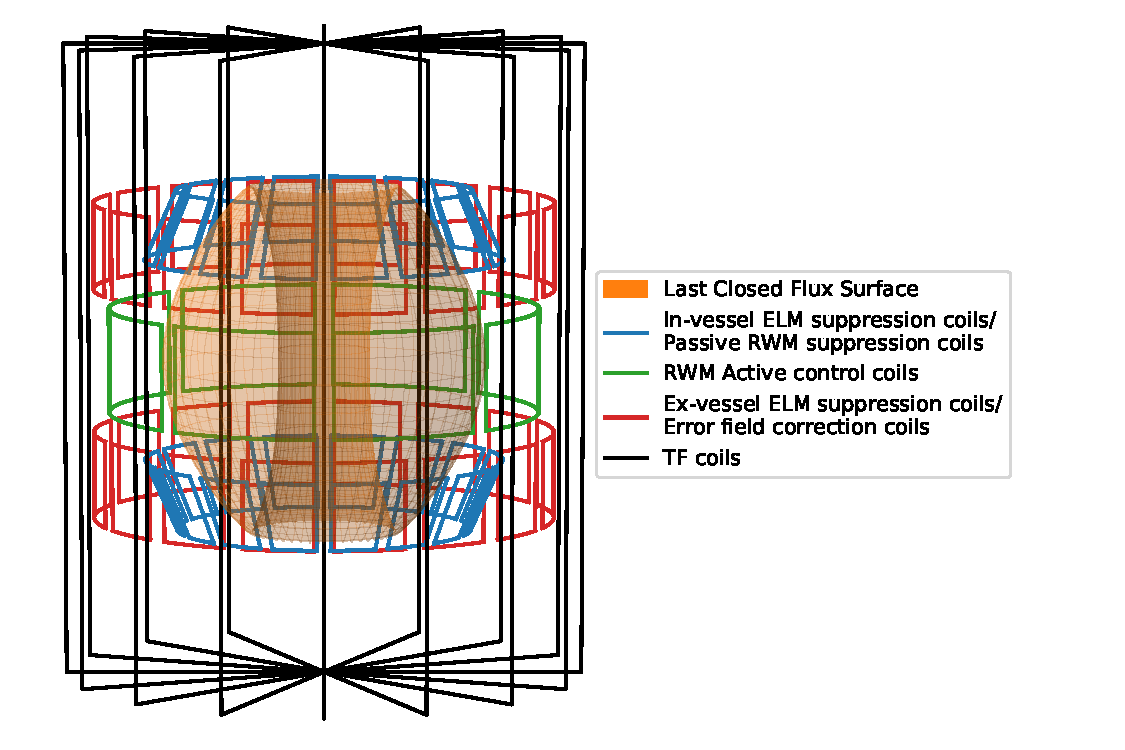
\includegraphics[width=0.8\linewidth]{Figures/coil_plot_3d.pdf}
    \caption{Schematic representation of STEP’s last closed flux surface, ELM suppression coils (which are interior and exterior to the vacuum vessel), RWM active control coils and TF coils. These designs are likely to change in the future. 
}
    \label{fig:coil_plot_3d}
\end{figure}

Fig. \ref{fig:max_and_total_flux_vs_rcoil_and_ncoil} shows the maximum energy flux on the walls and the total flux for different radii of the TF coils and the number of TF coils. The current design, with a major radius of approximately $\si{9.m}$ and 16 TF coils, has power losses that remain within acceptable limits. Increasing the radius of the coil or the number beyond these values will have a minimal effect on improving the confinement of the $\alpha$ particles. 
% Unfortunately, due to the need to fit other instruments such as the vacuum vessel, it is difficult to reduce the outer radius of the TF coil. The results also show that we can reduce the number of TF coils from 16 to 12 without affecting the confinment (assuming a radius of $9\si{.m}$ is maintained).
Unfortunately, it is difficult to save costs by reducing the outer radius of the TF coils due to the need to accommodate other essential elements such as the vacuum vessel, blanket, and PF (polodial field) coils. However, the results indicate that the number of TF coils could be reduced from 16 to 12 without compromising the confinement if a coil radius of $\si{9.m}$ were adopted.

\begin{figure}[!htb]
    \centering
    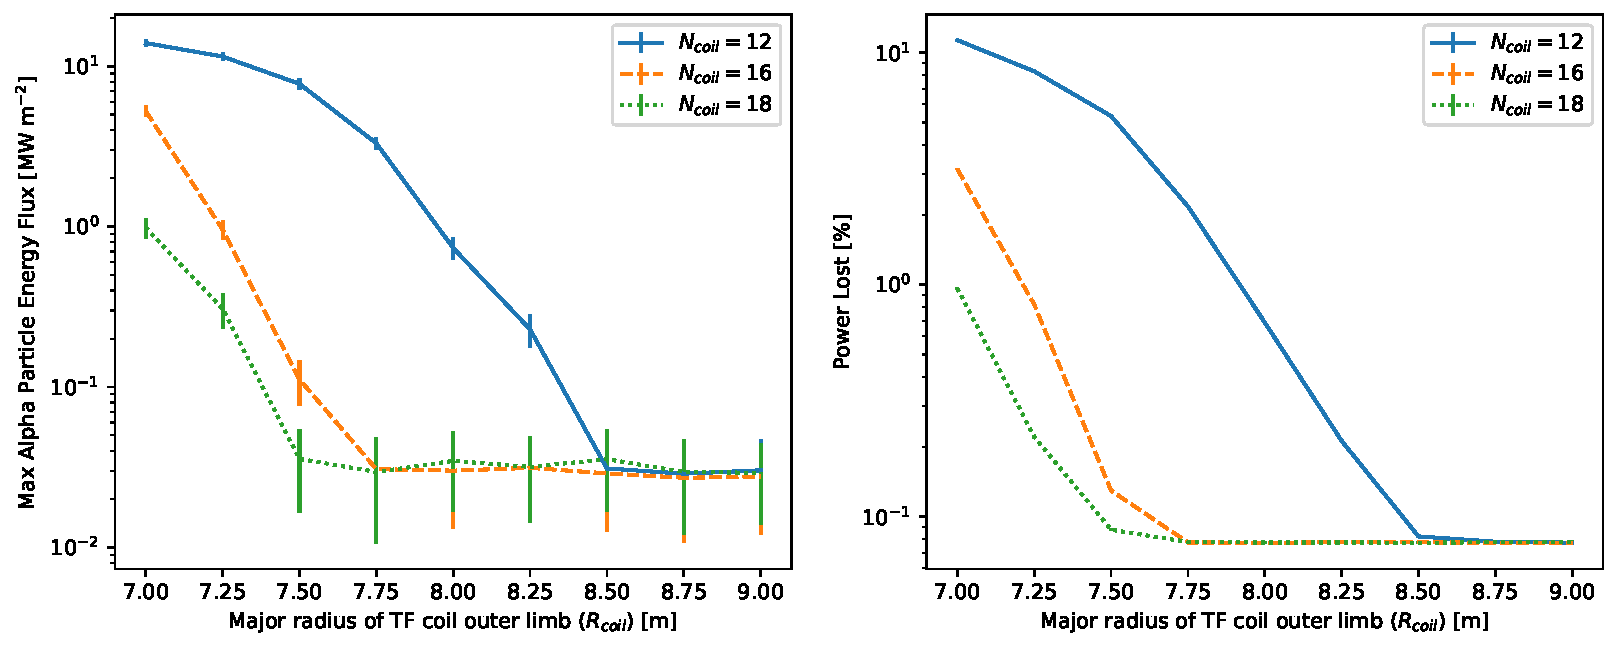
\includegraphics[width=0.99\linewidth]{Figures/max_and_total_flux_vs_rcoil_and_ncoil.pdf}
    \caption{TF ripple-induced losses for three values of $N_{coil}$ (the number of TF coils). The left plot shows the maximum energy flux on the reactor wall in $\si{MW.m^{-2}}$ and the right plot indicates the percentage of $\alpha$-particle power escaping and impacting the PFCs. Error bars represent 95\% confidence intervals, reflecting the statistical uncertainty inherent in the Monte Carlo methodology of the simulation. The black horizontal dotted line shows the results from a simulation where we used only the axisymmetric field.}
    \label{fig:max_and_total_flux_vs_rcoil_and_ncoil}
\end{figure}

\subsubsection{Internal and External ELM suppression fields}
\label{sec:elm_suppression_field}

In this section we model the confinement of $\alpha$-particles in the presence of ELM suppression fields.
% , excluding the TF ripple component (the latter has a minimal effect on the confinement in the most recent TF coil design). 
The ELM suppression field can be generated by coils that are inside the vacuum vessel (see blue coils in Fig. \ref{fig:coil_plot_3d}) or external to the vacuum vessel (see red coils in Fig. \ref{fig:coil_plot_3d}). Ex-vessel coils are currently favoured since it may be challenging to provide sufficient cooling to the in-vessel coils. Nevertheless, a definitive conclusion on which coil set will be used has not been reached, so we will analyse both scenarios in this study.

There are sixteen of each type of ELM suppression coil in each row, as illustrated in Figure \ref{fig:coil_plot_3d}. The current in the $k^\text{th}$ coil of the upper and lower rows is given by
\begin{align}
    \label{eq:ELM_coilcurrent_profile_upper}
    I_k^{upper} &= I_0 \cos(n \phi_k + \Delta \phi), \\
    \label{eq:ELM_coilcurrent_profile_lower}
    I_k^{lower} &= I_0 \cos(n \phi_k)
\end{align}
where $k$ ranges from 1 to 16, $I_0$ is the maximum current value, $\phi_k$ is the toroidal angle of the centre of the $k^\text{th}$ coil, $n$ is the principal toroidal mode number chosen to be excited, and $\Delta \phi$ is a free parameter that provides a phase shift. This produces a magnetic field that can be expressed as
\begin{equation}
    \delta\textbf{B}^\text{ELM}(R, \phi, z)=\Re\qty[\qty(\delta\textbf{B}^\text{ELM}_\text{real}(R,z) + i\delta\textbf{B}^\text{ELM}_\text{imag}(R,z))\exp(in\phi)].
\end{equation}
Other toroidal harmonics (sidebands) are present, but they have a sufficiently small amplitude that their effect on $\alpha$-particle confinement can be ignored when 16 ELM suppression coils are used. However, if only 8 coils are employed, the sidebands cannot be ignored. The magnetic fields arising from these currents are, in general, modified as a result of their interaction with the plasma. Plasma reaction is more prominent for lower toroidal mode numbers ($n$) \cite{mcclements2005}. For the ripple field, the toroidal is mode large enough that we can neglect the plasma response. For the suppression of ELMs, we plan to set $n=3$. Higher values of $n$ decay more quickly with distance from the coils, decreasing their efficacy, while lower values of $n$ may activate locked modes. Nevertheless, the choice of $n$ may change, and so we also model the cases with $n=2$ and $n=4$. To model the plasma response, we used the MARS-F code \cite{liu2015}. It is difficult to confirm the accuracy of the plasma response calculations and so we will also analyse the results for the case where the vacuum ELM suppression field is used.

% Equation \ref{eq:ELM_coilcurrent_profile} has three adjustable parameters: the toroidal mode number ($n$), the amplitude ($I_0$), and the phase shift $\Delta \phi$.
We have calculated the optimal values of $\Delta \phi = \Delta \phi_{opt}$, which maximise a quantity denoted by $\abs{b^1_{res}}$. This is a dimensionless measure of the field perturbation perpendicular to a resonant flux surface. We choose a flux surface very close to the separatrix, at $q=10$, as the one at which $\abs{b^1_{res}}$ is maximised. 
% as this is the outermost surface that is resonant for all values of $n=2$, 3, 4. 
Note that $\abs{b^1_{res}}$ gives a measure of the displacement of the X-point \cite{ryan2017}. In \cite{suttrop2018}, the authors showed that $\abs{b^1_{res}}=10^{-4}$ was sufficient to suppress ELMs in ASDEX Upgrade. The authors in \cite{liu2015} hypothesise that a similar value of $\abs{b^1_{res}}=10^{-4}$ will be needed to suppress ELMs for ITER. Extrapolating from the aforementioned ASDEX Upgrade results, we hypothesise that a value $\abs{b^1_{res}}=10^{-4}$ will be needed to suppress ELMs for STEP. However, since this is an extrapolation, we will also model the fast ion losses in scenarios where $\abs{b^1_{res}}$ is greater than $10^{-4}$. We present the optimal phase shifts ($\Delta \phi_{opt}$) and the corresponding coil currents required to ensure $\abs{b^1_{res}}=10^{-4}$ in Table \ref{table:optimum_currents_and_phases}. 
\begin{table}[h]
\centering
\begin{tabular}{lccc}
\hline
 & \( n=2 \) & \( n=3 \) & \( n=4 \) \\
\hline
In-Vessel ELM suppression coil current [kAt] & 30 & 50 & 80 \\
Ex-Vessel ELM suppression coil current [kAt] & 50 & 90 & 150 \\
In-Vessel ELM suppression coil \(\Delta\phi_{opt}\) [degrees] & 265 & 173 & 67 \\
Ex-Vessel ELM suppression coil \(\Delta\phi_{opt}\) [degrees] & 61 & 20 & 321 \\
\hline
\end{tabular}
\caption{Current in kAt required to exceed \( b^1_{res} > 10^{-4} \), and optimal coil phases.}
\label{table:optimum_currents_and_phases}
\end{table}

To suppress ELMs, $I_0$ must be large enough, but not so large that it reduces $\alpha$-particle confinement to an unacceptable extent. Given the uncertainty on the current required to suppress ELMs we will model the $\alpha$-particle losses with the currents quoted in Table \ref{table:optimum_currents_and_phases} and twice these values.
% Experiments on ASDEX Upgrade, when extrapolated to STEP, suggest that for $n=2$, a current of 50 kAt would be necessary, for $n=3$ a current of 90 kAt would be required, and for $n=4$ a current of 150 kAt would be needed. However, there is a high degree of uncertainty over the current needed, so we also model coil currents with twice these values. 
We model the $\alpha$-particle losses with the phase shifts $\Delta\phi_{opt}$ shown in Table \ref{table:optimum_currents_and_phases}. Additionally, we analyse the impact of changing the phase shift $\Delta\phi$ of the current profile of the upper coil set in comparison to the lower set on the confinement of fast particles. We consider $\Delta\phi$ values of $0^\circ$, $45^\circ$, $90^\circ$, $135^\circ$, $180^\circ$, $225^\circ$, $270^\circ$, and $315^\circ$. It should be noted that the $\Delta\phi$ used here is equal to $360^{\circ}-\Delta\phi^{\prime}$ where $\Delta\phi^{\prime}$ is the phase shift referred to in papers that report MARS-F modelling of RMPs, for example \cite{ryan2017}   

Fig. \ref{fig:max_and_total_flux_vs_phase_elm_rwm} and \ref{fig:max_and_total_flux_vs_phase_elm} show the predicted maximum flux of $\alpha$-particle energy on the first wall of STEP and the percentage of $\alpha$-power lost. As in the TF ripple simulations, we assume 1.7 GW of fusion power (hence $\sim\si{338.MW}$ of $\alpha$-particle power). The results are highly sensitive to the phase shift, as observed experimentally in ASDEX Upgrade \cite{sanchis2018}. These two figures also show that the losses are generally greater when the plasma response to the ELM suppression field is taken into account. However even when larger coil currents are used and the plasma response is included, acceptable heat loads can be achieved ($\ll \si{1.MW.m^{-2}}$) for suitably-chosen values of the phase shift. The findings suggest that better confinement can be achieved for $n=3$ and $n=4$ than for $n=2$. This could be due to the fact that the amplitudes of higher $n$ modes fall off more rapidly with distance from the coils, thus reducing the field perturbations in the plasma core where the great majority of high energy $\alpha$-particles are located.

\begin{figure}[!htb]
    \centering
    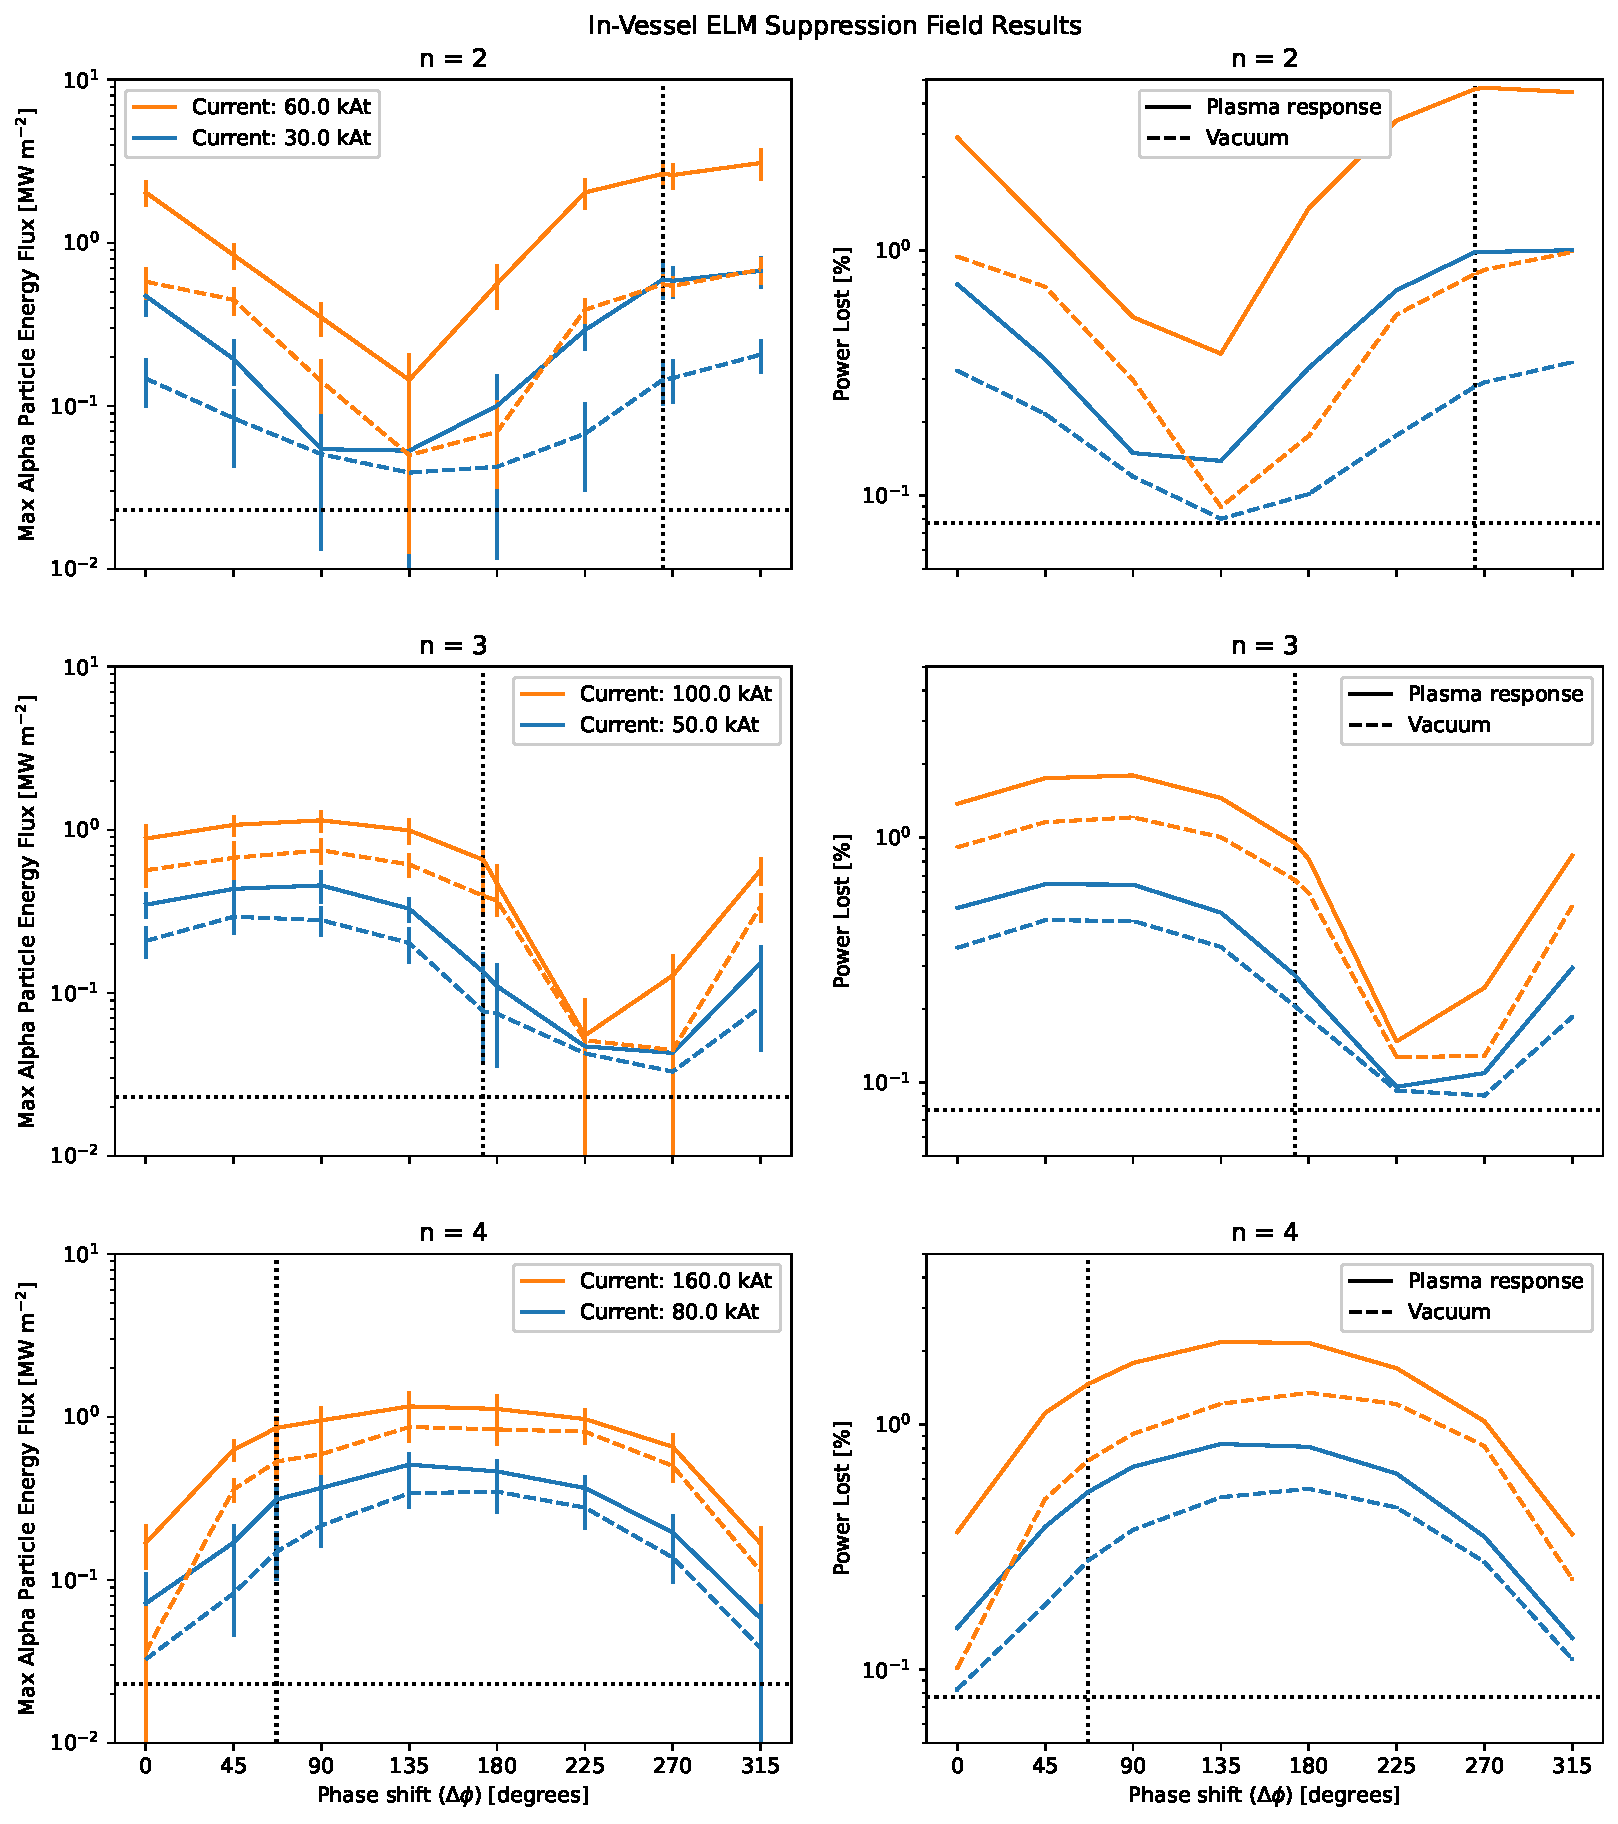
\includegraphics[width=0.99\linewidth]{Figures/max_and_total_flux_vs_phase_rwm.pdf}
    \caption{Maximum energy flux (left plots) and percentage heating power lost (right plots) due to deconfined $\alpha$-particles versus ELM suppression coil current phase shift $\Delta\phi$ for different values of $n$ and $I_0$ when in-vessel coils are used. Dashed curves were obtained with vacuum fields, while solid curves show the losses when the plasma response to the perturbations was included. The horizontal dotted line shows results from a simulation in which only the axisymmetric field was used, and the vertical dotted line gives the optimum phase $\Delta \phi_{opt}$ for ELM suppression.}
    \label{fig:max_and_total_flux_vs_phase_elm_rwm}
\end{figure}

\begin{figure}[!htb]
    \centering
    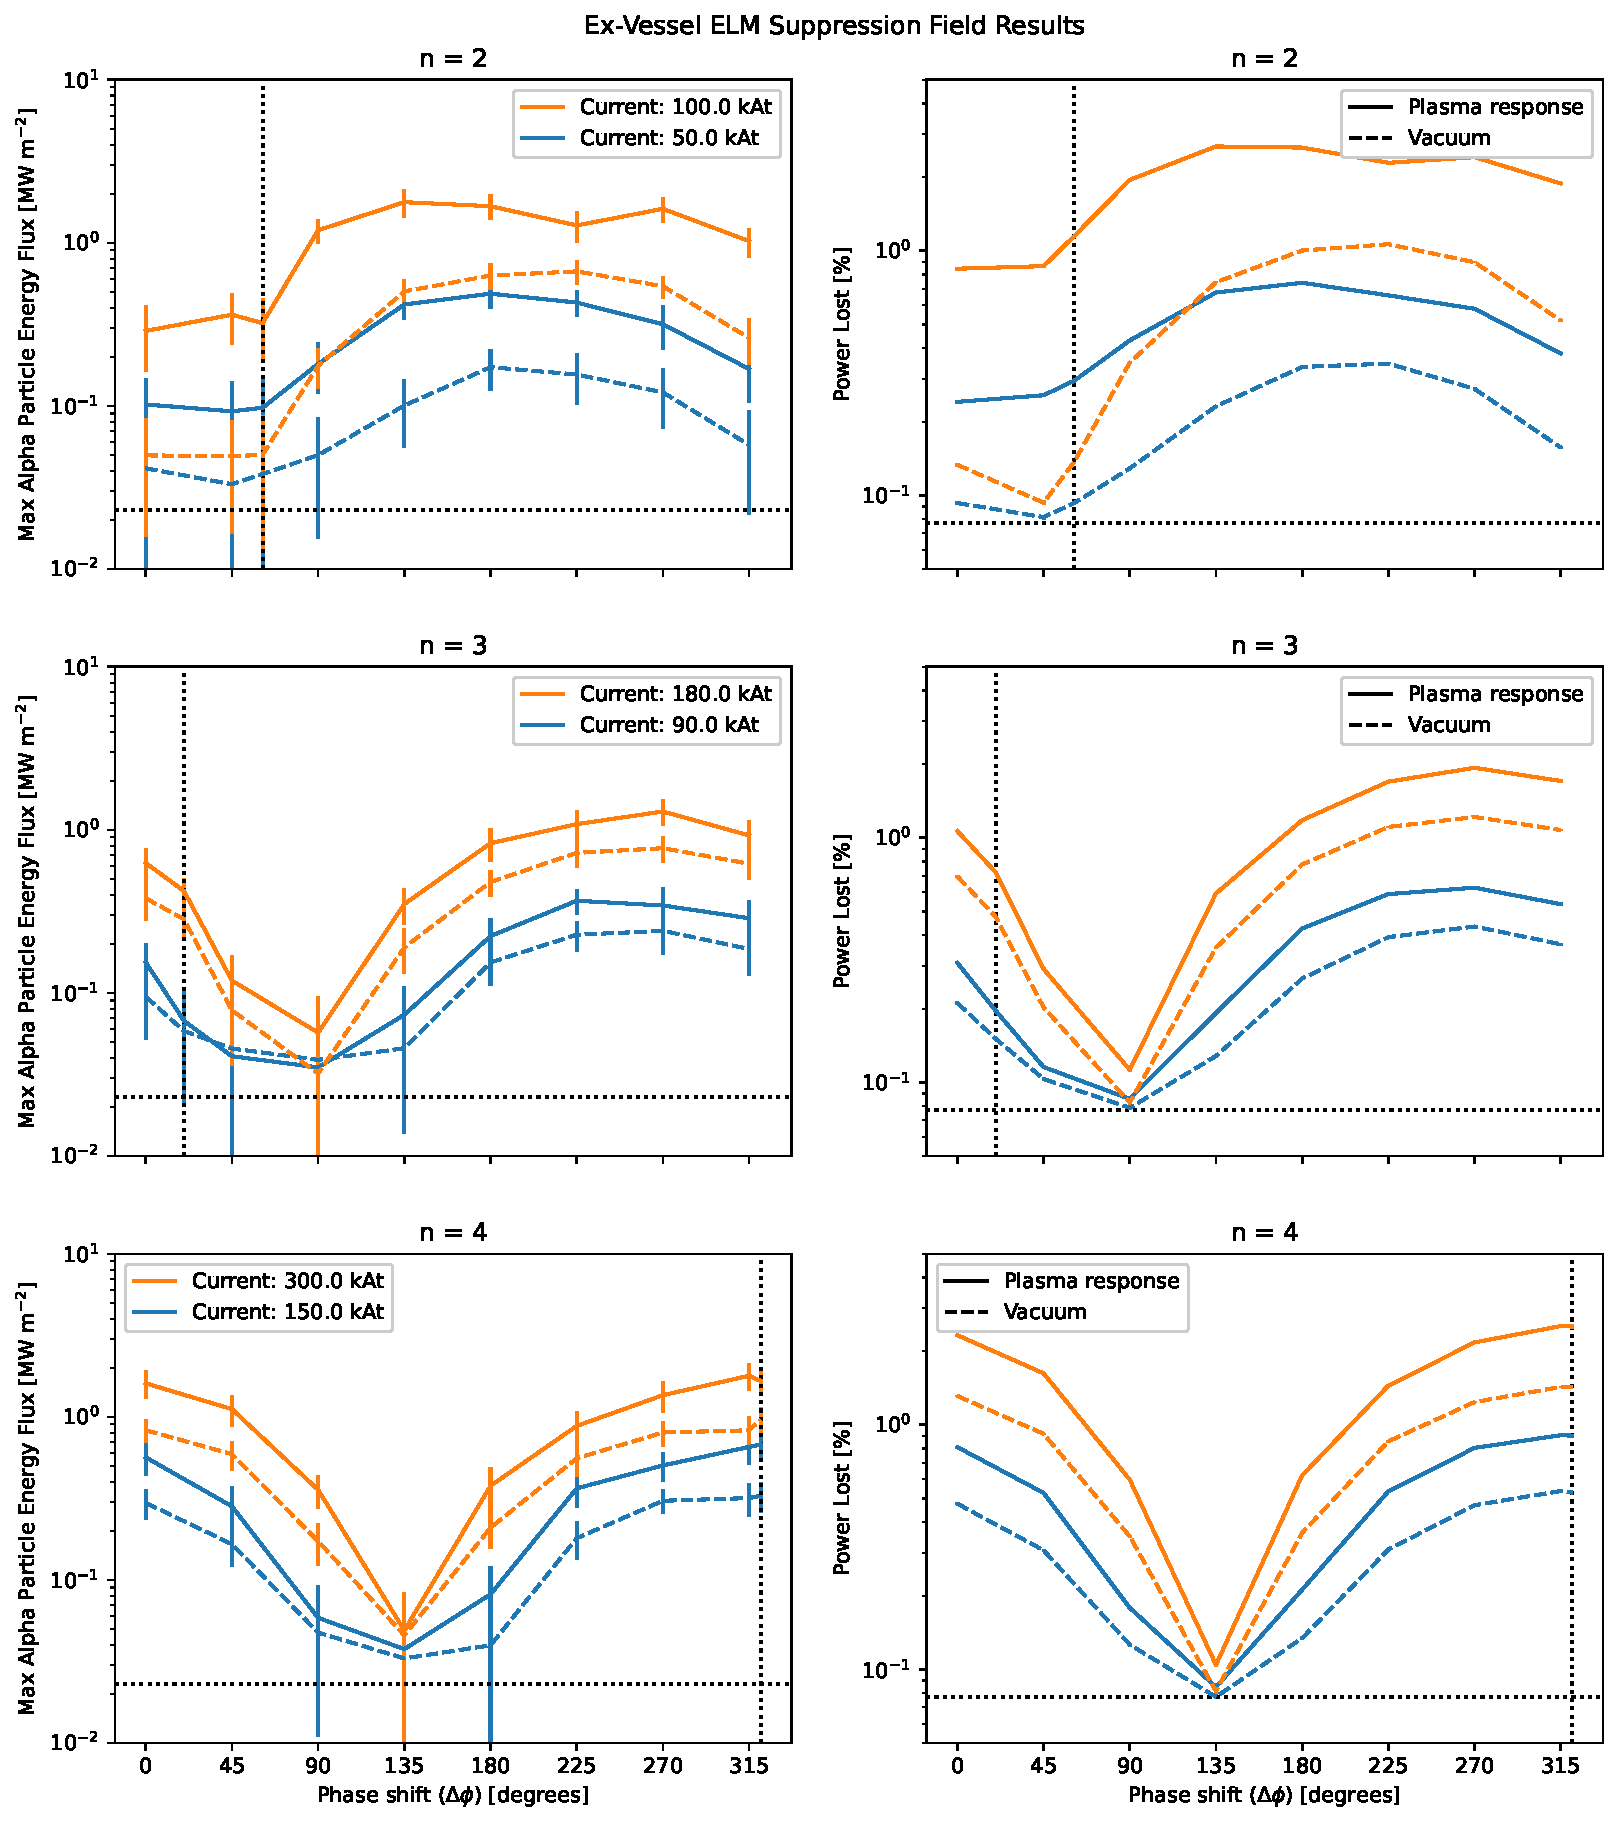
\includegraphics[width=0.99\linewidth]{Figures/max_and_total_flux_vs_phase_efcc.pdf}
    % \caption{Caption}
    % \caption{\parbox{0.9\linewidth}{This figure shows the results from 96 simulations. The left-columns s on the wall in $\si{MW.m^{-2}}$}}
    \caption{As Fig. \ref{fig:max_and_total_flux_vs_phase_elm_rwm} except that ex-vessel coils are employed to suppress ELMs in this case.}
    \label{fig:max_and_total_flux_vs_phase_elm}
\end{figure}

% The optimal $\Delta\phi$ for ELM suppression has been estimated using MARS-F \textbf{cite paper} by applying the criterion that the normalised field perturbation in the plasma should exceed $10^{-4}$: this has been found to be required for effective ELM control in current experiments. In the case of $n = 3$, with the plasma response included, it has been found that ELM suppression is favoured when $\Delta\phi \sim 180^{\circ}$, a value that is somewhat greater than the optimum for minimising $\alpha$-particle losses ($\sim 90^{\circ}$) in this case (see middle row of Fig. \ref{fig:max_and_total_flux_vs_phase_elm}). The choice of $\Delta\phi$ may thus require a compromise between the requirements of ELM suppression and acceptably low $\alpha$-particle losses.

\subsubsection{Poloidal distribution of RMP-induced heat loads}

In Fig. \ref{fig:energy_flux_distribution} we show the variation with poloidal angle of heat loads due to $\alpha$-particle losses in one of the more likely RMP scenarios, with $n=3$, $I_0= \si{90.kAt}$, $\Delta \phi = 20^\circ$ and with the plasma response included. More precisely, Fig. \ref{fig:energy_flux_distribution} shows how the $\alpha$-particle energy flux maximised over toroidal angle $S_{max}$ varies with poloidal distance along the first wall, $s_\theta$:
\begin{equation}
    \label{eq:max_alpha_particle_energy_flux}
    S_{max}(s_\theta) = \max_{0\le \phi \le 2\pi}\qty{S(\phi, s_\theta)},
\end{equation}
where $S=S(\phi, s_\theta)$ denotes the $\alpha$-particle energy flux on the first wall.
In the right-hand plot of Fig. \ref{fig:energy_flux_distribution}, the boundaries between the outboard and inboard main chamber walls and the upper and lower divertor regions are marked by vertical lines in blue, orange, green, and red. These are labeled with the symbols +, $\times$, $\bullet$, and $\blacksquare$ respectively. The corresponding symbols and colours are also shown in the left plots for reference. These results show that the largest energy flux is on the dome in the upper divertor, with another significant peak at the end of the outer leg in the lower divertor. As mentioned previously, the maximum tolerable heat loads in these regions are, respectively, around 5 MWm$^{-2}$ and 10 MWm$^{-2}$: the values plotted in Fig. \ref{fig:energy_flux_distribution} are well within these limits. 

\begin{figure}[!htb]
    \centering
    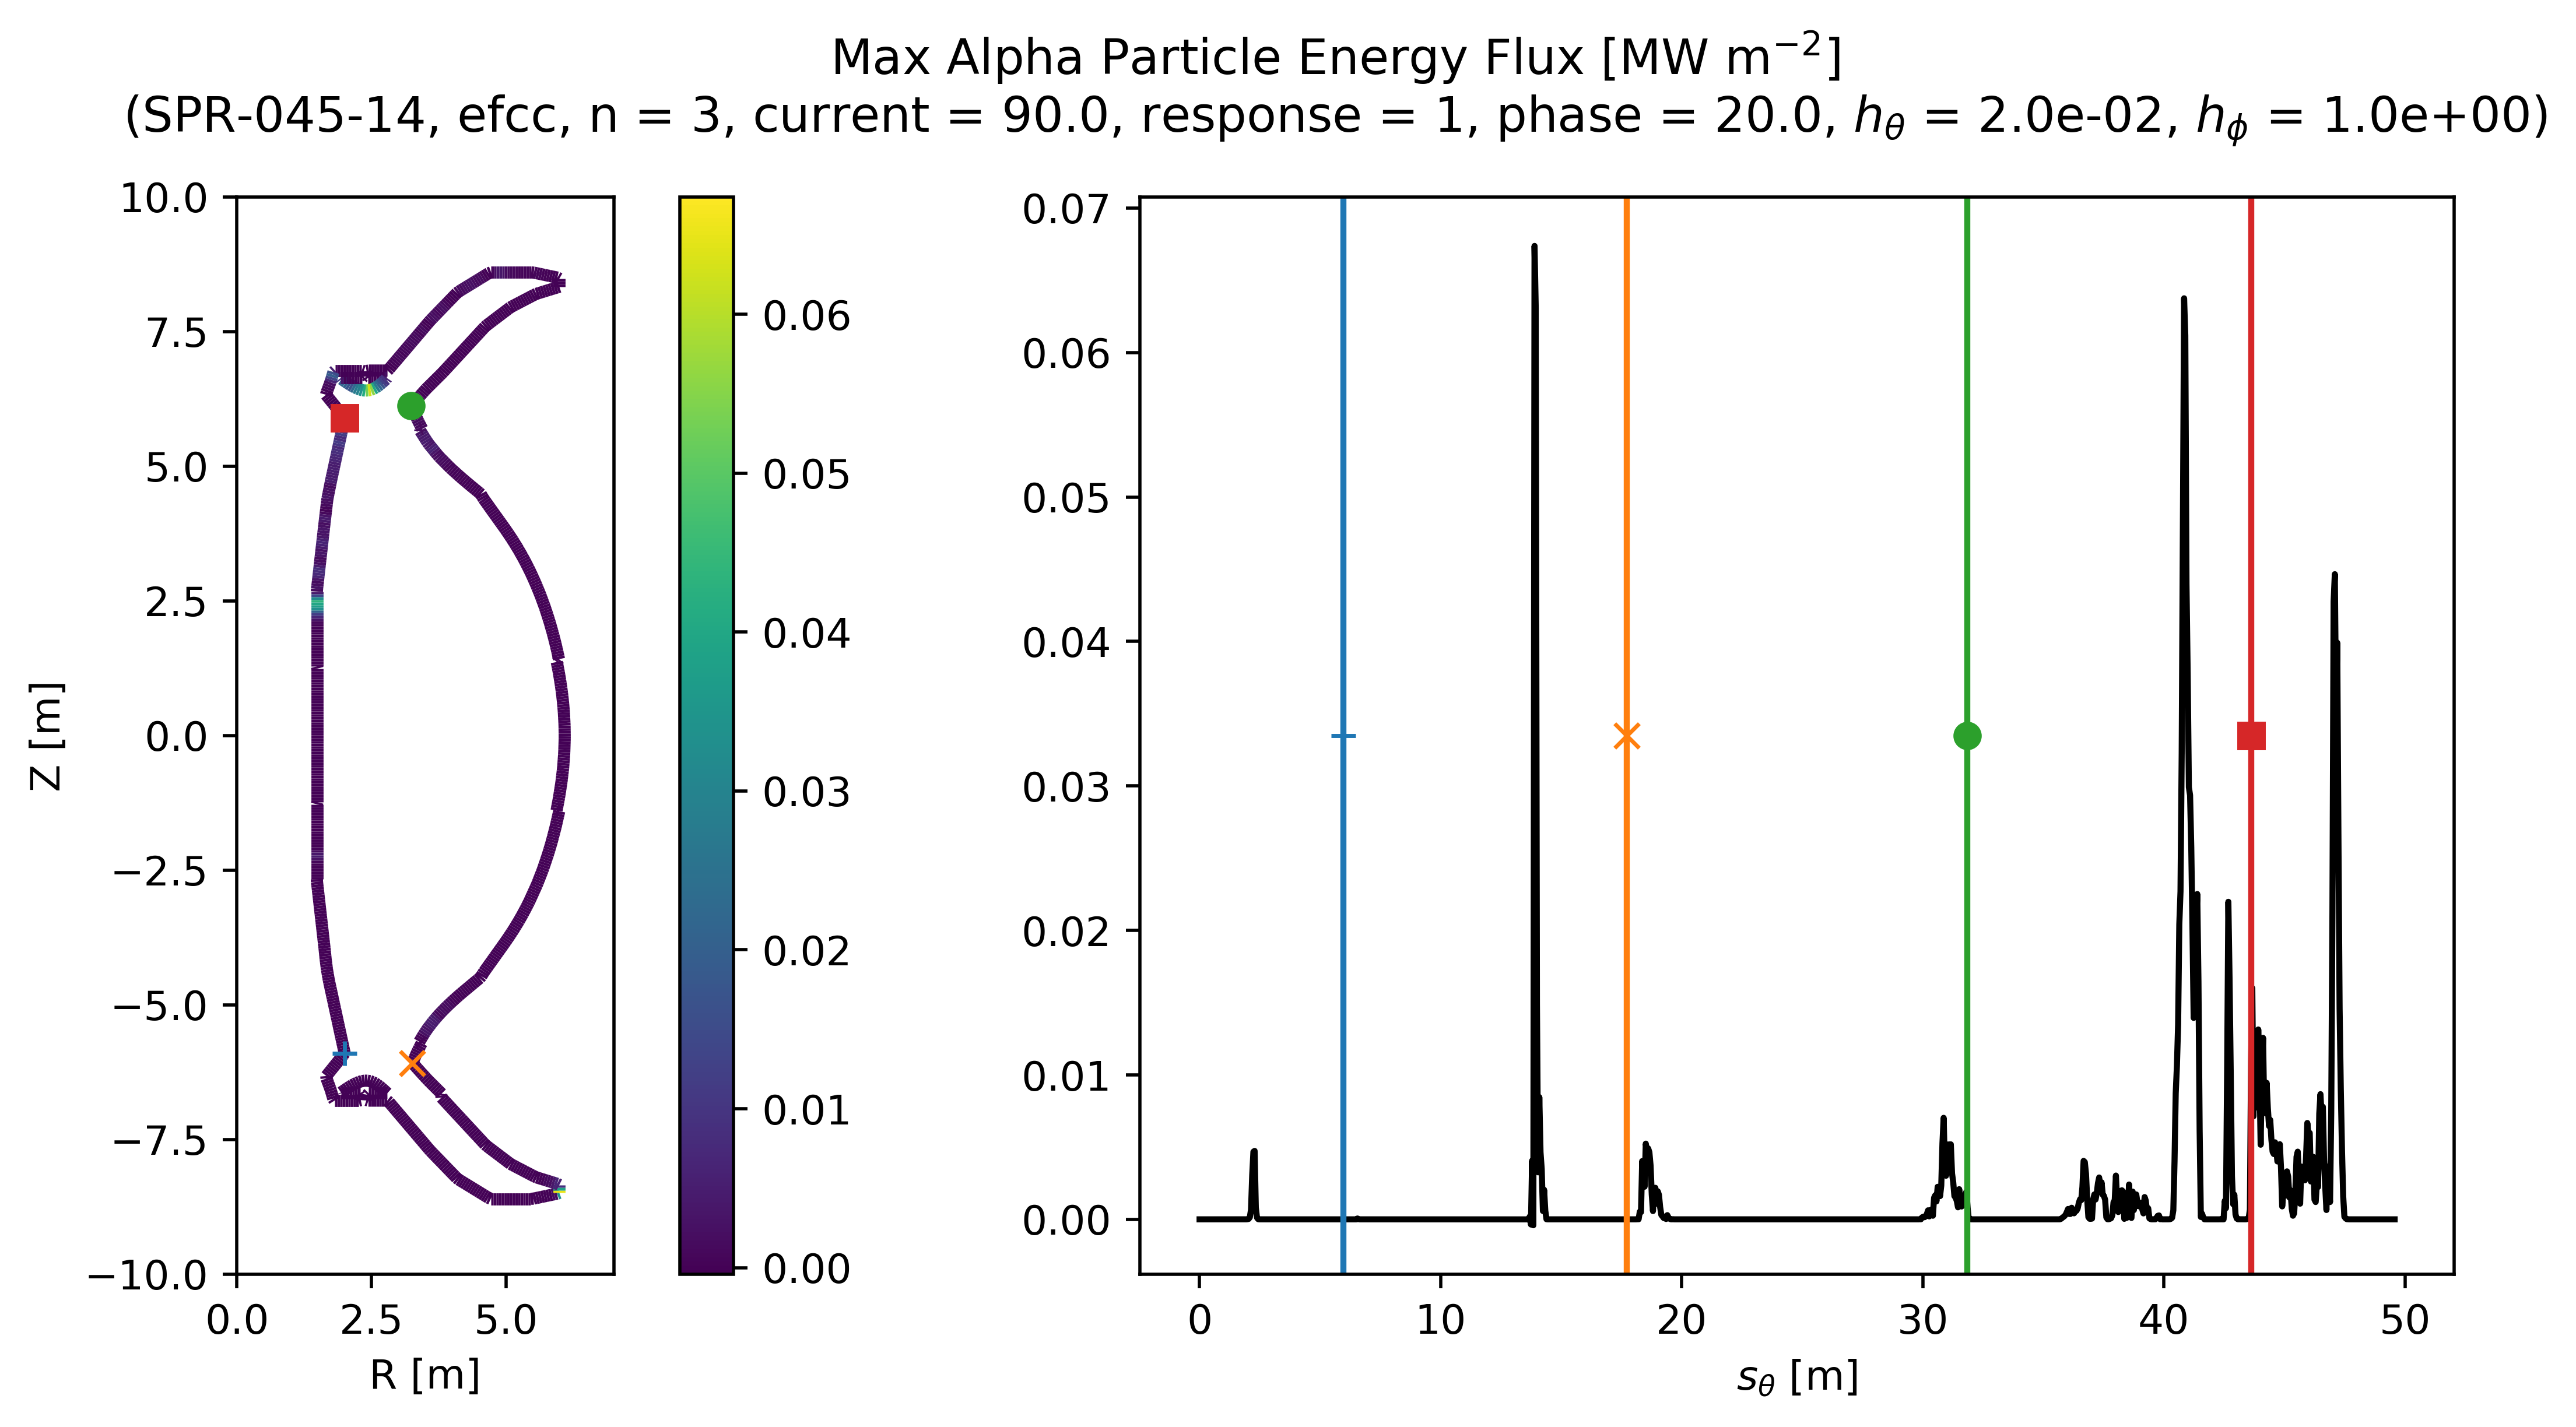
\includegraphics[width=0.99\linewidth]{Figures/simple_line_plot_no_confidence_band.png}
    \caption{Distribution of peak $\alpha$-particle energy flux maximised over toroidal angle in poloidal cross-section (left) and versus poloidal distance $s_\theta$ along the wall (right plot). Both graphs display the maximum alpha particle energy flux, denoted as $S_{max}$, measured in $\si{MW.m^{-2}}$. The definition of $S_{max}$ can be found in Equation \eqref{eq:max_alpha_particle_energy_flux}.}
    \label{fig:energy_flux_distribution}
\end{figure}

\subsubsection{RWM field}
\label{sec:rwm_field}

To maximise fusion power, it is intended that STEP will operate above the no-wall beta limit for $n=1$ resistive wall modes (RWMs). This means that both active feedback and passive control of RWMs will be required \cite{xia2023}. The active feedback coils are activated once the RWM amplitude surpasses a predefined threshold, set at 1 G in the latest design.
Sensors are located near the active control coils (see Figure \ref{fig:coil_plot_3d}), measuring the field intensity and initiating the feedback cycle in response.

In Fig. \ref{fig:max_and_total_flux_vs_bscale_rwm} we present the results of simulations in which an RWM of fixed amplitude is present. 
We use MARS-F to solve an eigenvalue problem to identify the poloidal structure of the RWM \cite{xia2023}. Since this is a linear calculation, the perturbation amplitude is a free variable.
In \cite{xia2023}, the authors model the RWM and the response of the active feedback coils, including the effects of noise from the sensor signal, in their results. The feedback coils stop the growth of the RWMs, but for any finite noise level there is a residual $n=1$ perturbation in the plasma. The amplitude at the sensor can reach more than ten times the threshold value, meaning that the field there can be as high as 10 G. In the present paper we only model the RWM and will not include the modification to the field due to the feedback system. We leave the modelling of the full-time-evolving field as a topic for future study. We investigate the scenarios in which the magnitude of the signal detected by the sensors is 1 G, 10 G, 100 G and 1000 G (i.e. $\si{10^{-4}.T}$, $\si{10^{-3}.T}$, $\si{10^{-2}.T}$ and $\si{10^{-1}.T}$ respectively). The results in Fig. \ref{fig:max_and_total_flux_vs_bscale_rwm} indicate that even if the RWM is allowed to reach 100 G at the sensors, the impact on the confinement of the $\alpha$-particles is minimal. If the amplitude of an RWM became so large that the magnitude of the signal detected by the sensors was 100 G or more, it would be likely to cause a disruption and our steady-state model would no longer be applicable. In such a scenario deconfined high energy $\alpha$-particles could pose a threat to plasma facing components in addition to that arising from runaway electrons, but we do not consider such effects here. 

\begin{figure}[!htb]
    \centering
    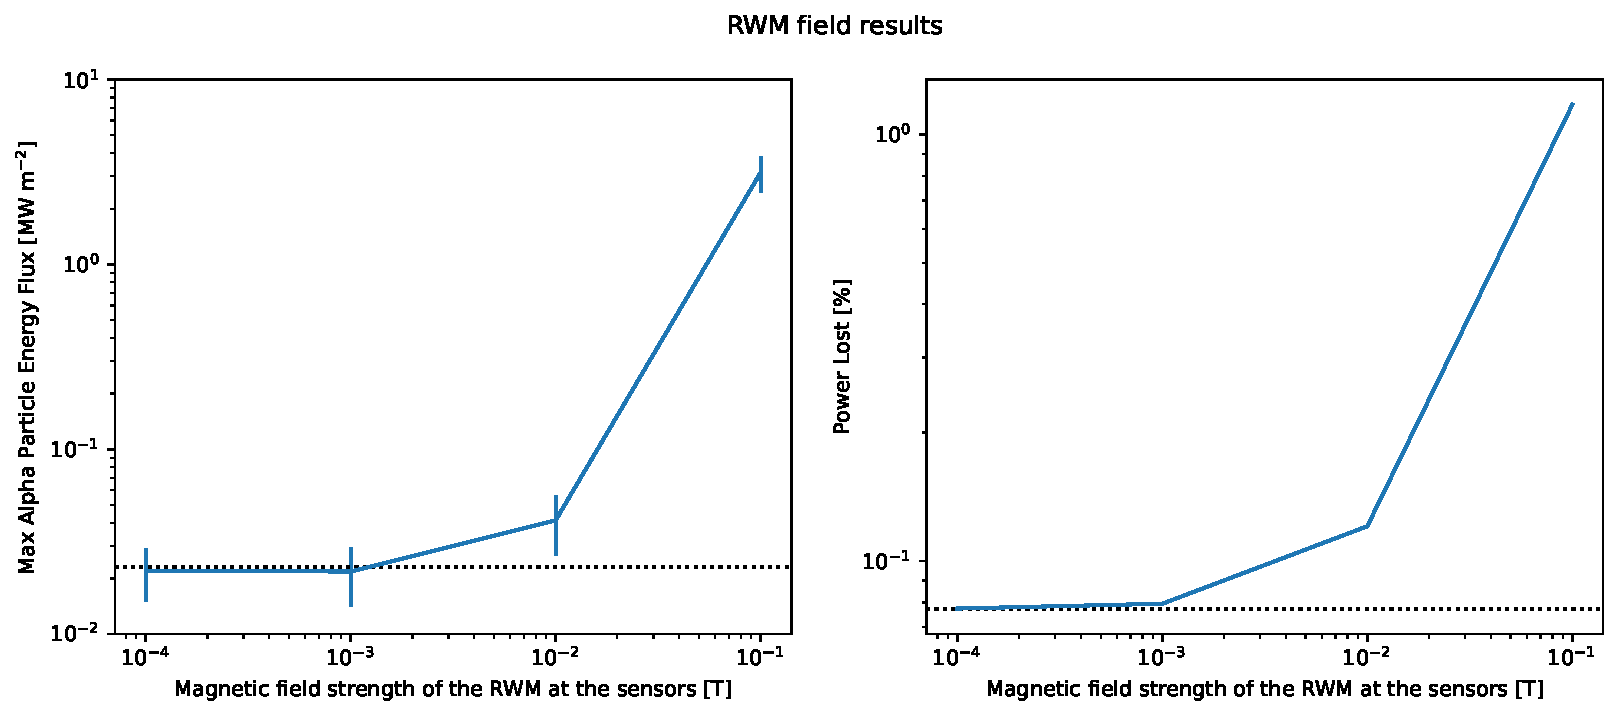
\includegraphics[width=0.99\linewidth]{Figures/max_and_total_flux_vs_bscale_rwm.pdf}
    \caption{Maximum energy flux (left plot) and percentage heating power lost (right plot) due to deconfined $\alpha$-particles versus RWM amplitude at the sensors located near the RWM control coils. In this case the only non-axisymmetric field is that arising from the RWM. The results in the axisymmetric limit are again shown by dotted horizontal lines.}
    \label{fig:max_and_total_flux_vs_bscale_rwm}
\end{figure}

% Resistive Wall Modes (RWMs) are expected to appear in STEP. To address this, we plan to use RWM coils to generate magnetic fields, allowing active and passive control of RWMs, as described in \cite{xia2023}. Since these RWM fields are three-dimensional, there is a potential for a major effect on the confinement of $\alpha$-particles. Our aim is to thoroughly examine the effects of RWM coils on the $\alpha$-particles and to incorporate these results in our comprehensive submission to the Nuclear Fusion journal. We plan to use 8 RWM coils in each row. Therefore, the sidebands, which were discussed in Section \ref{sec:elm_suppression_field}, will make up a significant part of the RWM field.

\section{TAE stability calculations}
\label{sec:halo_work}

TAEs are driven unstable due to wave-particle resonances, principally the Landau resonance, which occurs when the particle speed parallel to the magnetic field matches the Alfv\'en speed, $c_A$. The only trans-Alfv\'enic fast ions of any significance in STEP DT plasmas will be the $\alpha$-particles, born with an approximately isotropic velocity distribution clustered around a speed $\sim 1.3\times\si{10^7ms^{-1}}$. This is nearly an order of magnitude higher than the typical values of $c_A$ envisaged in STEP flat-top operation, and therefore the resonance condition will be satisfied by $\alpha$-particles as they slow down. However, although the intrinsic fast ion drive of TAEs is expected to be high in STEP, strong bulk plasma damping of these modes is also expected. The physical reason for this is that STEP will need to be a high plasma $\beta$ device to generate net electrical power, and local values of $\beta$ in the plasma core will be a substantial fraction of unity, meaning that the bulk ion thermal speed $v_i$ will be comparable to $c_A$. Moreover, in addition to the primary Landau resonance $v_{\parallel}=c_A$, in a toroidal plasma there are also sideband resonances $v_{\parallel} = c_A/\vert 2\ell-1 \vert$ where $\ell$ is a positive integer. As a result of these two effects, many bulk ions as well as fast ions can resonate with TAEs in STEP plasmas, and the interaction of bulk ions with these modes is generally expected to result in strong Landau damping.

The stability of TAEs in STEP has been studied using the HAGIS \cite{pinches1998} and HALO \cite{fitzgerald2020} codes. One particular STEP scenario is relatively compact with major radius $R_0 = 3.0\,$m, toroidal field $B_0 = 1.8\,$T and central fuel ion temperature $T_i(0)=17\,$keV. Intrinsic growth rates (i.e. $\alpha$-particle drive) of TAEs with a range of values of $n$ in the absence of all damping processes were calculated using HAGIS with the $\alpha$-particles modelled using slowing-down distributions: these growth rates are plotted in Fig. \ref{fig:TAEs}. It can be seen that most TAEs have normalised growth rates $\gamma/\omega$ of a few percent but one $n=2$ mode has much stronger drive, with $\gamma/\omega \simeq 0.18$. In this case, the mode electric field extends further into the plasma core than that of other modes and can thus interact with a high concentration of $\alpha$-particles deep inside the plasma. 

\begin{figure}[!htb]
    \centering
    \vskip -3.0cm
    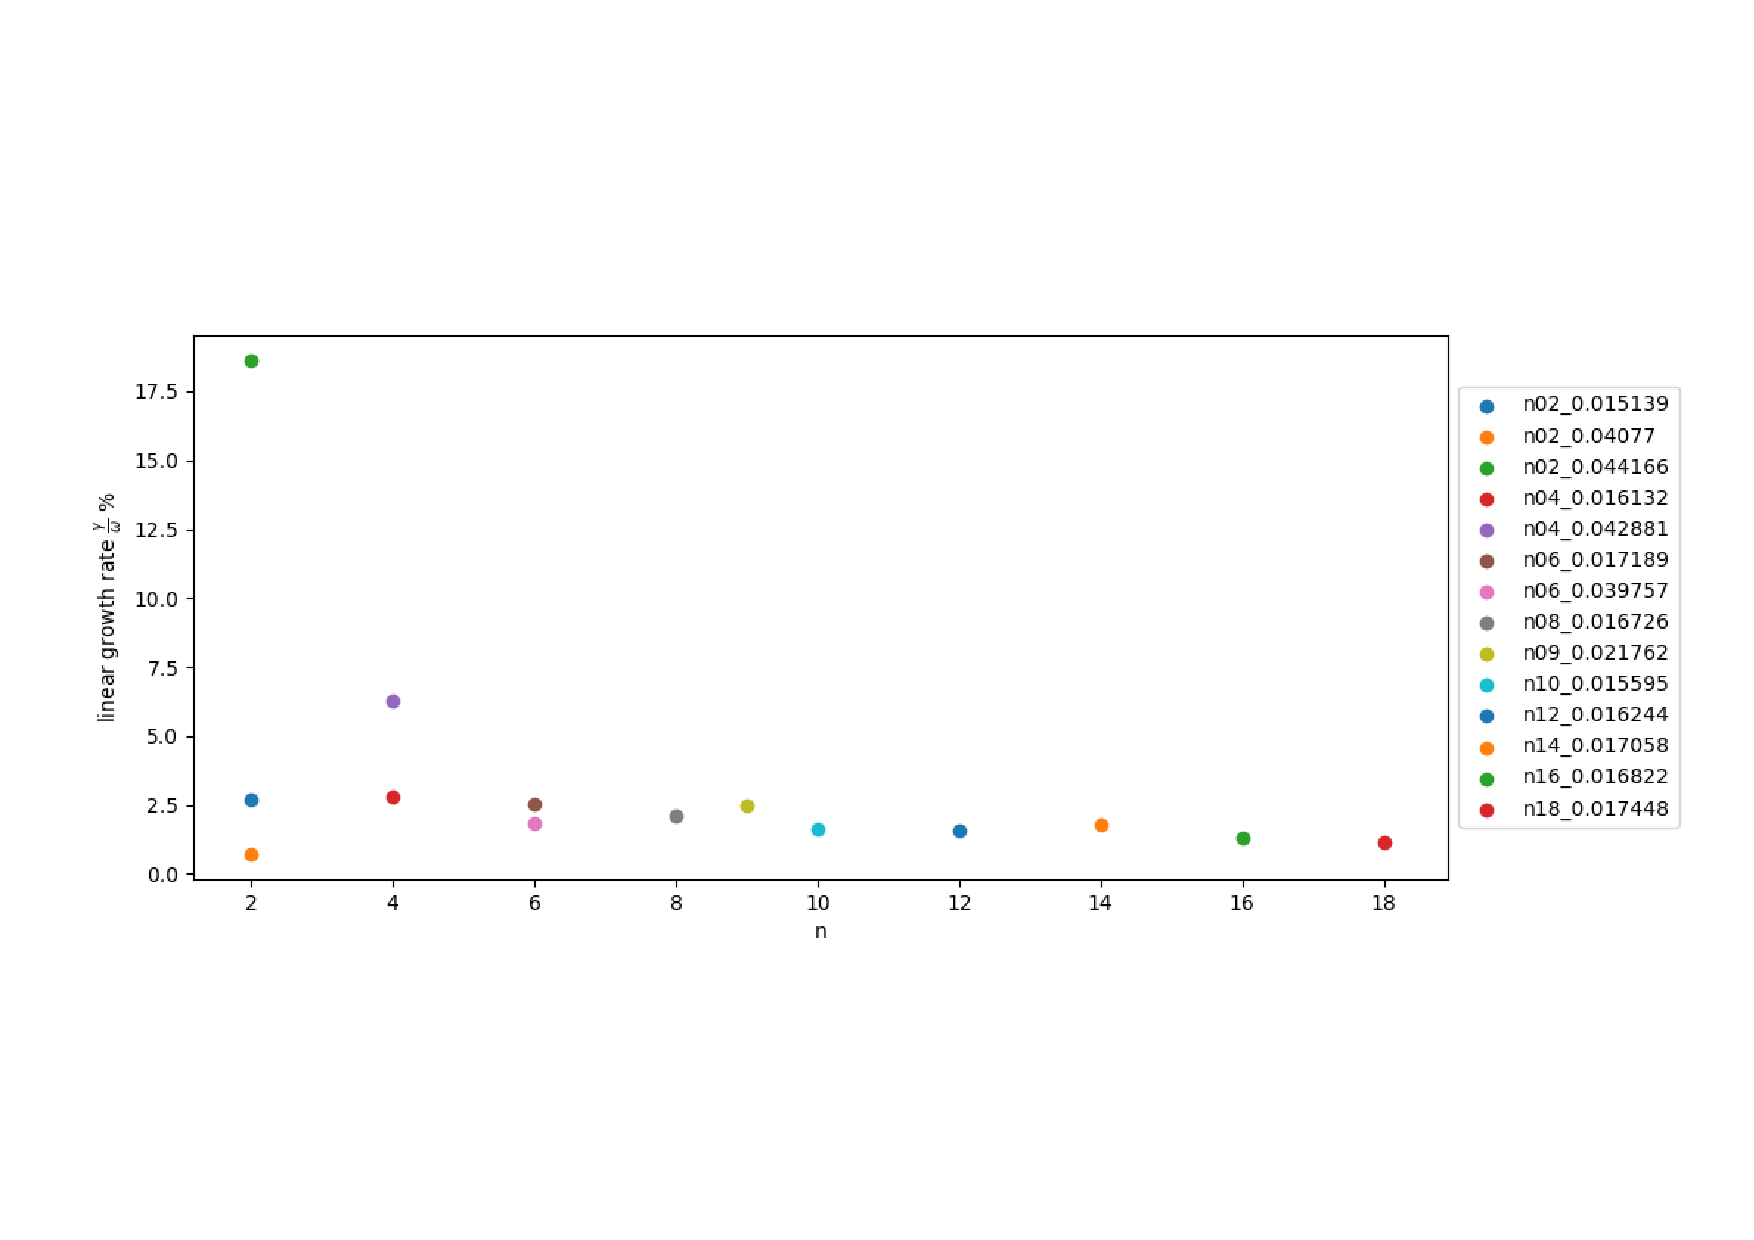
\includegraphics[width=1.0\linewidth]{Figures/TAE_figure.pdf}
    \vskip -3.0cm
    \caption{Growth rates of TAEs with damping neglected in equilibrium with $B_0 = 1.8\,$T, $T_i(0) = 17\,$keV computed using HAGIS. The legend indicates the mode $n$ and squared frequency normalised to $c_A/R_0$ where $c_A$ is the Alfv\'en speed at the magnetic axis, $R=R_0$.}
    \label{fig:TAEs}
\end{figure}

HALO calculations with Maxwellian bulk ions but without $\alpha$-particles indicate that the Landau bulk ion damping of this mode $\gamma_d$ is even stronger than the drive: we find $\gamma_d/\omega \simeq -1.4$. It should be noted that this damping rate is exponentially sensitive to the bulk-ion plasma beta, and therefore it is important to perform a sensitivity scan of the plasma parameters, in particular $B_0$ and $T_i(0)$. We find, however, that TAEs remain damped in other flat-top plasma scenarios studied so far and are therefore unlikely to pose a threat to $\alpha$-particle confinement during this phase of a STEP plasma pulse.        

\section{Discussion, conclusions and future study}
\label{sec:discussion_and_conclusions}

As expected, $\alpha$-particles in STEP are well confined in the axisymmetric limit, and TF ripple losses are acceptably low if there are 16 TF coils with outer limbs at major radii of at least $\si{8.m}$. Losses arising from the use of ELM suppression coils pose a more substantial challenge. Our work shows that a suboptimal choice of phase difference $\Delta\phi$ between the upper and lower sets of ELM coils can result in significant deterioration of $\alpha$-particle confinement, and the optimum $\Delta\phi$ for the suppression of ELMs in general differs from that for $\alpha$-particle confinement. However, the losses are within acceptable limits in terms of power load on the wall. More experimental research in spherical tokamaks and in double null devices is needed to establish the requirements for active suppression of ELMs in STEP. However, the work presented here provides useful information to inform the design process, giving us more confidence that a solution to the ELM problem can be found that is compatible with acceptable losses of $\alpha$ particles.

In Section \ref{sec:rwm_field} we studied the losses in a scenario where the magnetic field due to an RWM was included in the model and found that the losses were only slightly higher than the axisymmetric level, even when the perturbation reached a value of $\si{10^{-2}.T}$ at the RWM detector. This magnitude at the detector would be unacceptable, as it could potentially cause a disruption. Therefore, the results suggest that the RWMs, if kept controlled, will not be a problem for $\alpha$-particle losses. However, this analysis did not take into account the feedback from the RWM active control, which is a field that varies over time (see \cite{xia2023}) and could significantly modify the poloidal structure of the magnetic field. We intend to investigate the effect of the active control field in the near future, including also the effects of sensor noise and the plasma response to the field generated by the control coils. Additionally, we plan to validate our LOCUST simulation results by using the ASCOT code \cite{hirvijoki2014}.

% To maximise the fusion power, it is intended that STEP will operate above the no-wall beta limit for resistive wall modes (RWMs) with $n=1$. Active and passive control of RWMs will therefore be required \cite{xia2023}. When noise is taken into account, residual field perturbations with dominant $n=1$ are present during RWM control, and these perturbations have the potential to degrade $\alpha$-particle confinement. We therefore plan to model the effects of residual field perturbations due to dedicated RWM coil currents on $\alpha$-particle confinement. The most recent STEP design includes 8 RWM active control coils along the midplane. Toroidal sidebands, discussed in Section \ref{sec:elm_suppression_field}, will make up a significant part of the RWM field and will therefore need to be included in the LOCUST modelling.

Future research in the field of Alfv\'en eigenmode stability in STEP will focus {\it inter alia} on the potential destabilisation of these modes by fast electrons during the ramp-up phase (when the electron cyclotron current drive will be employed \cite{Henderson2024}) and by runaway electrons during disruptions. Additionally, the impact of the $q$-profile on Alfv\'en eigenmode stability during the flat-top phase will be explored. We also plan to check the stability of ellipticity-induced Alfv\'en eigenmodes and noncircular triangularity-induced Alfv\'en eigenmodes as well as TAEs. However, higher frequency compressional Alfv\'en eigenmodes are probably irrelevant to STEP since they are normally only driven by anisotropic fast ions \cite{Gorelenkov2016}, which will not be present. 

% In addition to our focus on the flat-top/steady-state phase, as mentioned in Section \ref{sec:introduction}, it is essential to determine if the $\alpha$-particles are adequately confined during the ramp-up and ramp-down phases.

% \textbf{For future work we intend to verify our results by collaborating with VTT to check ASCOT gives the same results.}

% \textbf{Number of ELM suppression coils in each row may be reduced from 16 to 8.}

\section*{Acknowledgements}

This work has been funded by STEP, a UKAEA program to design and build a prototype fusion energy plant and a path to commercial fusion.

% Format text for bibliography
% If more than three authors put et al.
\fontsize{9}{12}\selectfont
\setlength{\parskip}{0pt}
\begin{thebibliography}{9}

\bibitem{nuttall2020} % book chapter
% example: CHAPTER-AUTHOR, A., “Title of chapter in sentence case”, Book Title in Title Case, Publisher, Place of Publication (Year).
    WILSON, H., CHAPMAN, I., DENTON, T., et al., 
    ``STEP---on the pathway to fusion commercialization", 
    Commercialising Fusion Energy, 
    IOP Publishing, 
    (2020).

\bibitem{meyer2023} % poster at conference
% example: PRESENTER, A., “Title of presentation in sentence case”, Paper No., paper presented at Organization seminar on subject, Location, year.
    MEYER, H.,
    ``The plasma scenarios for the Spherical Tokamak for Energy Production (STEP) and their technical implications",
    29\textsuperscript{th} IAEA Fusion Energy Conference,
    poster presentation, 
    London, UK, 
    2023

%\bibitem{belova2015} % journal article
% example: AUTHOR, A., AUTHOR, B., AUTHOR, C., Journal article title in sentence case, Abb. J. Title 1 %2 (Year) 120–123.
%    BELOVA, E., GORELENKOV, N., FREDRICKSON, E., et al., 
%    Coupling of neutral-beam-driven compressional Alfv\'en eigenmodes to kinetic Alfv\'en waves in %NSTX tokamak and energy channeling, 
%    Phys. Rev. Lett. 
%    \textbf{115} 1 
%    (2015) 
%    015001.

\bibitem{mitchell2023} % journal article
% example: AUTHOR, A., AUTHOR, B., AUTHOR, C., Journal article title in sentence case, Abb. J. Title 1 2 (Year) 120–123.
    MITCHELL, J., PARROTT, A., CASSON, F., et al.,
    Scenario trajectory optimization and control on STEP,
    Fusion Eng. Des.
    \textbf{192} 
    (2023) 
    113777.

% \bibitem{zsolt2023} % internal report
% % example: AUTHOR, A., Internal Report Title in Title Case, internal report, Organization, Location, Year.
%     ZSOLT, V., et al., 
%     TD-001004, 
%     internal report, 
%     UKAEA, 
%     2023.

\bibitem{garcia-munoz2011} % journal article
% example: AUTHOR, A., AUTHOR, B., AUTHOR, C., Journal article title in sentence case, Abb. J. Title 1 2 (Year) 120–123.
    GARC\'IA-MU\~NOZ, M., CLASSEN, I.G.J., GEIGER, B., et al., 
    Fast ion transport induced by Alfv\'en eigenmodes in the ASDEX Upgrade tokamak, 
    Nucl. Fusion 
    \textbf{51} 
    (2015) 
    103013.

\bibitem{Henderson2024} % journal article
% example: PRESENTER, A., “Title of presentation in sentence case”, Paper No., paper presented at Organization seminar on subject, Location, year.
    HENDERSON, M., FREETHY, S., CRAIG, S., et al., 
    The concept design of the STEP heating and current drive system,
    Nucl. Fusion
    submitted, 
    2024

\bibitem{bachmann2018} % internal report
% example: AUTHOR, A., Internal Report Title in Title Case, internal report, Organization, Location, Year.
    BACHMANN, C., CIATTAGLIA, S., CISMONDI, F., et al., 
    Overview over DEMO design integration challenges and their impact on component design concepts, 
    Fusion Eng. Des. 
    \textbf{136} 
    (2018)
    87.

%\bibitem{fil2023} % poster at conference
% example: PRESENTER, A., “Title of presentation in sentence case”, Paper No., paper presented at %Organization seminar on subject, Location, year.
%    FIL, A., HENDEN, L., NEWTON, S., et al.,
%    ``Disruption runaway electron generation and mitigation in the Spherical Tokamak for Energy %Production",
%    poster presentation, 
%    29\textsuperscript{th} IAEA Fusion Energy Conference,
%    London, UK, 
%    2023

\bibitem{Berger2022} % journal article
% example: PRESENTER, A., “Title of presentation in sentence case”, Paper No., paper presented at Organization seminar on subject, Location, year.
    BERGER, E., PUSZTAI, I., NEWTON, S., et al.,
    ``Runaway dynamics in reactor-scale spherical tokamak disruptions",
    J. Plasma Phys. 
    \textbf{88} 6 
    (2022)
    905880611.

\bibitem{zohm1996} % journal article
% example: AUTHOR, A., AUTHOR, B., AUTHOR, C., Journal article title in sentence case, Abb. J. Title 1 2 (Year) 120–123.
    ZOHM, H., 
    Edge localized modes (ELMs), 
    Plasma Phys. Control. Fusion 
    \textbf{38} 2 
    (1996) 
    105.

\bibitem{xia2023} % journal article
% example: AUTHOR, A., AUTHOR, B., AUTHOR, C., Journal article title in sentence case, Abb. J. Title 1 2 (Year) 120–123.
    XIA, G., LIU, Y., HENDER, T., et al.,
    Control of resistive wall modes in the spherical tokamak,
    Nucl. Fusion,
    \textbf{63} 2
    (2023)
    026021.

% \bibitem{wagner1982} % journal article
% % example: AUTHOR, A., AUTHOR, B., AUTHOR, C., Journal article title in sentence case, Abb. J. Title 1 2 (Year) 120–123.
%     WAGNER, F., BECKER, G., BEHRINGER, K., et al., 
%     Regime of improved confinement and high beta in neutral-beam-heated divertor discharges of the ASDEX tokamak, 
%     Phys. Rev. Lett. 
%     \textbf{49} 19
%     (1982) 
%     1408.

\bibitem{Evans2008} % journal article
% example: AUTHOR, A., AUTHOR, B., AUTHOR, C., Journal article title in sentence case, Abb. J. Title 1 2 (Year) 120–123.
    EVANS, T., FENSTERMACHER, M., MOYER, R., et al.,
    RMP ELM suppression in DIII-D plasmas with ITER similar shapes and collisionalities,
    Nucl. Fusion,
    \textbf{48} 1 
    (2008) 
    096031.

\bibitem{suttrop2018} % journal article
% example: AUTHOR, A., AUTHOR, B., AUTHOR, C., Journal article title in sentence case, Abb. J. Title 1 2 (Year) 120–123.
    SUTTROP, W., KIRK, A., BOBKOV, V., et al.,
    Experimental conditions to suppress edge localised modes by magnetic perturbations in the ASDEX Upgrade tokamak,
    Nucl. Fusion,
    \textbf{58} 9 
    (2018) 
    096031.

\bibitem{In2019} % journal article
% example: AUTHOR, A., AUTHOR, B., AUTHOR, C., Journal article title in sentence case, Abb. J. Title 1 2 (Year) 120–123.
    IN, Y., LOARTE, A., LEE, H., et al.,
    Test of the ITER-like resonant magnetic perturbation configurations for edge-localized mode crash suppression on KSTAR,
    Nucl. Fusion,
    \textbf{59} 12 
    (2019) 
    096031.
    
\bibitem{van2015} % journal article
% example: AUTHOR, A., AUTHOR, B., AUTHOR, C., Journal article title in sentence case, Abb. J. Title 1 2 (Year) 120–123.
    VAN ZEELAND, M., FERRARO, N., GRIERSON, B., et al.,
    Fast ion transport during applied 3D magnetic perturbations on DIII-D,
    Nucl. Fusion,
    \textbf{55} 7,
    (2015)
    073028.

\bibitem{sanchis2018} % journal article
% example: AUTHOR, A., AUTHOR, B., AUTHOR, C., Journal article title in sentence case, Abb. J. Title 1 2 (Year) 120–123.
    SANCHIS, L., GARCIA-MUNOZ, M., SNICKER, A., et al.,
    Characterisation of the fast-ion edge resonant transport layer induced by 3D perturbative fields in the ASDEX Upgrade tokamak through full orbit simulations,
    Plasma Phys. Control. Fusion,
    \textbf{61} 1,
    (2018)
    014038.
    
\bibitem{ward2022} % journal article
% example: AUTHOR, A., AUTHOR, B., AUTHOR, C., Journal article title in sentence case, Abb. J. Title 1 2 (Year) 120–123.
    WARD, S., AKERS, R., LI, L., et al.,
    LOCUST-GPU predictions of fast-ion transport and power loads due to ELM-control coils in ITER,
    Nucl. Fusion,
    \textbf{62} 12
    (2022)
    126014.

\bibitem{akers2018} % poster at conference
    % example: PRESENTER, A., “Title of presentation in sentence case”, Paper No., paper presented at Organization seminar on subject, Location, year.
    AKERS, R., COLLING, B., HESS, J., et al.,
    ``High fidelity simulations of fast ion power flux driven by 3D field perturbations on ITER",
    poster presentation, 
    26\textsuperscript{th} IAEA Fusion Energy Conference,
    Kyoto, Japan, 
    2016.

\bibitem{ward2021} % journal article
% example: AUTHOR, A., AUTHOR, B., AUTHOR, C., Journal article title in sentence case, Abb. J. Title 1 2 (Year) 120–123.
    WARD, S., AKERS, R., JACOBSEN, A., et al.,
    Verification and validation of the high-performance Lorentz-orbit code for use in stellarators and tokamaks (LOCUST),
    Nucl. Fusion,
    \textbf{61} 8
    (2021)
    086029.

\bibitem{bosch1992} % journal article
% example: AUTHOR, A., AUTHOR, B., AUTHOR, C., Journal article title in sentence case, Abb. J. Title 1 2 (Year) 120–123.
    BOSCH, H., HALE, G.,
    Improved formulas for fusion cross-sections and thermal reactivities,
    Nucl. Fusion,
    \textbf{32} 4
    (1992)
    611-631.

\bibitem{brysk1973} % journal article
% example: AUTHOR, A., AUTHOR, B., AUTHOR, C., Journal article title in sentence case, Abb. J. Title 1 2 (Year) 120–123.
    BRYSK, H.,
    Fusion neutron energies and spectra,
    Plasma Phys.,
    \textbf{15} 7
    (1973)
    611-617.

\bibitem{chen2017} % journal article
% example: AUTHOR, A., AUTHOR, B., AUTHOR, C., Journal article title in sentence case, Abb. J. Title 1 2 (Year) 120–123.
    CHEN, Yen-Chi,
    A tutorial on kernel density estimation and recent advances,
    Biostat. Epidemiol,
    \textbf{1} 1
    (2017)
    161-187.

\bibitem{mcclements2005} % journal article
% example: AUTHOR, A., AUTHOR, B., AUTHOR, C., Journal article title in sentence case, Abb. J. Title 1 2 (Year) 120–123.
    MCCLEMENTS, K.,
    Full orbit computations of ripple-induced fusion $\alpha$-particle losses from burning tokamak plasmas,
    Phys. of Plasmas,
    \textbf{12} 7
    (2005)
    072510.

% \bibitem{ryan2022} % internal report
% % example: AUTHOR, A., Internal Report Title in Title Case, internal report, Organization, Location, Year.
%     RYAN, D., 
%     TD-0014685, 
%     internal report, 
%     UKAEA, 
%     2022.

\bibitem{liu2015} % journal article
% example: AUTHOR, A., AUTHOR, B., AUTHOR, C., Journal article title in sentence case, Abb. J. Title 1 2 (Year) 120–123.
    LIU, Y., AKERS, R., CHAPMAN, I., et al.,
    Modelling toroidal rotation damping in ITER due to external 3D fields,
    Nucl. Fusion,
    \textbf{55} 6
    (2015)
    063027.

\bibitem{ryan2017} % journal article
% example: AUTHOR, A., AUTHOR, B., AUTHOR, C., Journal article title in sentence case, Abb. J. Title 1 2 (Year) 120–123.
    RYAN, D. A., LIU, Y.Q., LI, L., et al.,
    Numerically derived parametrisation of optimal RMP coil phase as a guide to experiments on ASDEX Upgrade,
    Plasma Phys. Control. Fusion,
    \textbf{59} 2 
    (2017) 
    024005.

\bibitem{pinches1998} % journal article
% example: AUTHOR, A., AUTHOR, B., AUTHOR, C., Journal article title in sentence case, Abb. J. Title 1 2 (Year) 120–123.
    PINCHES, S.D., APPEL, L.C., CANDY, J., et al.,
    The HAGIS self-consistent nonlinear wave-particle interaction model,
    Computer Phys. Commun.
    \textbf{111}
    (1998)
    133.

\bibitem{fitzgerald2020} % journal article
% example: AUTHOR, A., AUTHOR, B., AUTHOR, C., Journal article title in sentence case, Abb. J. Title 1 2 (Year) 120–123.
    FITZGERALD, M., BUCHANAN, J, AKERS, R.J., et al.,
    HALO: a full-orbit model of nonlinear interaction of fast particles with eigenmodes,
    Computer Phys. Commun.
    \textbf{252}
    (2020)
    106773.

\bibitem{hirvijoki2014} % journal article
% example: AUTHOR, A., AUTHOR, B., AUTHOR, C., Journal article title in sentence case, Abb. J. Title 1 2 (Year) 120–123.
    HIRVIJOKI, E., ASUNTA, O., KOSKELA, T., et al.,
    ASCOT: Solving the kinetic equation of minority particle species in tokamak plasmas,
    Comput. Phys. Commun.,
    \textbf{185} 4 
    (2014) 
    1310-1321.

\bibitem{Gorelenkov2016} % journal article
% example: AUTHOR, A., AUTHOR, B., AUTHOR, C., Journal article title in sentence case, Abb. J. Title 1 2 (Year) 120–123.
    GORELENKOV, N.N.,
    Energetic particle-driven compressional Alfv\'en eigenmodes and prospects for ion cyclotron emission studies in fusion plasmas,
    New J. Phys.,
    \textbf{18}
    (2016) 
    105010.

\end{thebibliography}


\end{document}
